\documentclass{standalone}
\usepackage{pgfplots}
\usepackage{lmodern}
\pgfplotsset{compat=1.17}

\begin{document}
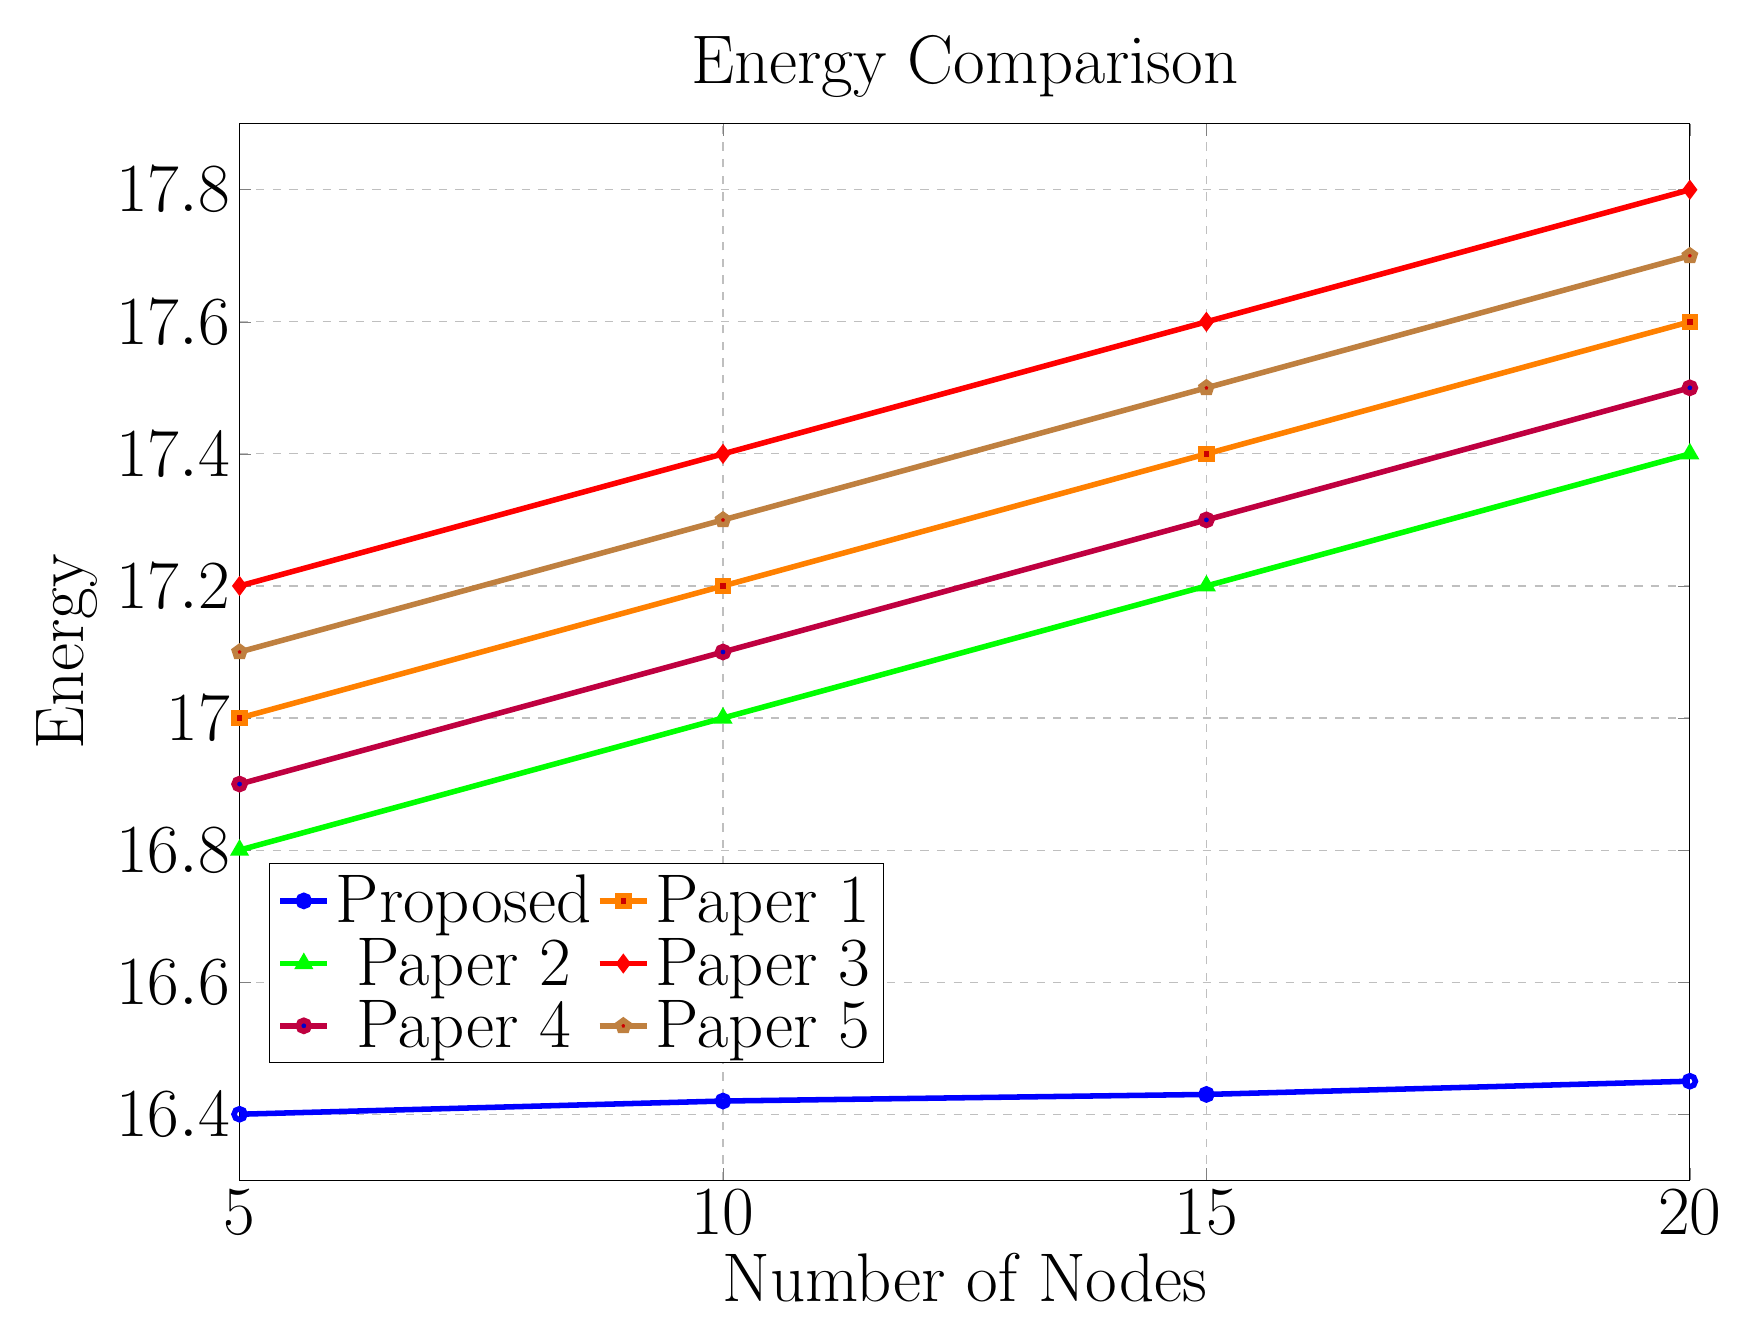
\begin{tikzpicture}
\begin{axis}[
 width=20cm,
 height=15cm,
 tick label style={font=\fontsize{24}{28}\selectfont},
 label style={font=\fontsize{24}{28}\selectfont},
 title style={font=\fontsize{24}{28}\selectfont},
 title={Energy Comparison},
 xlabel={Number of Nodes},
 ylabel={Energy},
 xmin=5, xmax=20,
 ymin=16.3, ymax=17.9,
 xtick={5,10,15,20},
 ytick={16.4,16.6,16.8,17.0,17.2,17.4,17.6,17.8},
 legend columns=2,
 legend style={
 font=\fontsize{24}{28}\selectfont,
 at={(0.02,0.3)},
 anchor=north west,
 draw=black,
 fill=white
 },
 ymajorgrids=true,
 xmajorgrids=true,
 grid style=dashed
]

% Proposed
\addplot+[mark=o,color=blue,line width=2pt] coordinates {
 (5,16.4)(10,16.42)(15,16.43)(20,16.45)
};

% Paper 1
\addplot+[mark=square*,color=orange,line width=2pt] coordinates {
 (5,17.0)(10,17.2)(15,17.4)(20,17.6)
};

% Paper 2
\addplot+[mark=triangle*,color=green,line width=2pt] coordinates {
 (5,16.8)(10,17.0)(15,17.2)(20,17.4)
};

% Paper 3
\addplot+[mark=diamond*,color=red,line width=2pt] coordinates {
 (5,17.2)(10,17.4)(15,17.6)(20,17.8)
};

% Paper 4
\addplot+[mark=*,color=purple,line width=2pt] coordinates {
 (5,16.9)(10,17.1)(15,17.3)(20,17.5)
};

% Paper 5
\addplot+[mark=pentagon*, color=brown, line width=2pt, solid] coordinates {
 (5,17.1)(10,17.3)(15,17.5)(20,17.7)
};

\legend{Proposed, Paper 1, Paper 2, Paper 3, Paper 4, Paper 5}

\end{axis}
\end{tikzpicture}
\end{document}